\chapter{Grundlagen}
\section{Usability}
\textit{Usability} in der Software-Entwicklung ist ein Qualitätsmaß, anhand dessen eine Einschätzung über die Einfachheit der Bedienung einer Benutzeroberfläche ermöglicht wird \cite{Nielsen2012}. Umgangssprachlich wird der Begriff \enquote{Benutzerfreundlichkeit} als deutsches Synonym verwendet. Betrachtet man jedoch den Wortstamm genauer, bemerkt man, dass die englische Vokabel aus zwei einzelnen Wörtern besteht. Dies ist zum einen \enquote{use} (engl. benutzen) und zum anderen \enquote{ability} (engl. die Möglichkeit). 

Nach Nielsen wird die Qualität einer Anwendung hinsichtlich der Usability durch 5 Kernaspekte bestimmt:
\begin{itemize}
	\item Erlernbarkeit
	\item Effizienz
	\item Einprägsamkeit
	\item Fehlertoleranz
	\item Zufriedenheit \cite{Nielsen2012}
\end{itemize}
Alle diese Aspekte können zu einer guten Gebrauchstauglichkeit beitragen. Eine hohe Erlernbarkeit ist gegeben, wenn der Dialog zwischen der Maschine und dem Anwender einfach gestaltet ist, sodass die Bedienung schnell erlernt werden kann. Es ist hilfreich, Designkonzepte zu verwenden, die dem Anwender aus anderen Anwendungen oder aus der Natur vertraut sind \cite[Learnability]{UsabilityFirstGlossary}. Auch die Erfüllung psychologischer Grundsätze (siehe Kap. \ref{sec:uxdPsychology} und Kap. \ref{sec:uidRules}) ist ein wichtiger Faktor. Ein effizienter Dialog erlaubt es dem Nutzer, seine Ziele möglichst schnell zu erreichen. Kurze Ladezeiten und wenige zur Problemlösung benötigte Interaktionen fördern die Effizienz. Einprägsam ist eine Software, wenn ein Nutzer nach längerer Nicht-Benutzung dieser, ohne viel Zeitaufwand, den professionellen Umgang damit wieder erlernen kann \cite{Nielsen2012}. Bei der Fehlertoleranz geht es darum, dass die Anwendung fehlerhafte Eingaben erkennt und behandeln kann. Entweder kann die Anwendung den Fehler kompensieren und bereinigen oder der Nutzer muss über die Fehleingabe informiert werden und die Gelegenheit bekommen, korrekte Eingaben zu machen. Da bei der Usability stets der Nutzer im Fokus der Entwicklung steht, ist es von entscheidender Bedeutung, diesen zufrieden zu stellen. Ein gutes Design, das eine angenehme Bedienung ermöglicht, hilft dabei \cite{Nielsen2012}. \par

\section{User-Experience Design} \label{sec:uxd}
Der Begriff \textit{User-Experience} (kurz: UX) beschreibt das Nutzungsempfinden einer Person, wenn Sie mit einem System interagiert. Der Ausdruck ist meist im Bereich der Mensch-Computer-Interaktion vorzufinden, beschränkt sich aber nicht auf diesen. \cite{Gube2010} So kann der Begriff auch auf andere Produkte, wie z.B. Mikrowellen, Brettspiele oder ganze Produktreihen (vgl. Microsoft Office Produkte) angewandt werden. Im Rahmen dieser Arbeit wird jedoch nur der Teilbereich der Mensch-Computer-Interaktion im Rahmen einer einzelnen Anwendung betrachtet. \par
Im Gegensatz zur Usability berücksichtigt die UX die Erwartungshaltung des Nutzers und versucht, ein angenehmes Gesamtbild der Anwendung und der Interaktion mit dieser zu vermitteln. Das Ziel des User-Experience Designs ist es nicht nur, eine hohe Produktivität zu ermöglichen, vielmehr versucht sie, die Interaktion zu einem Erlebnis zu machen, das dem Anwender positiv in Erinnerung bleibt. Dies geht sogar so weit, dass der UX-Designer beschließt, dem Nutzer unter Umständen Funktionalitäten vorzuenthalten, um das Erlebnis zu sichern \cite{Thielsch2015}. Als Beispiel führt Thielsch den \textit{Drift-Table} an. Bei dem Drift-Table handelt es sich um einen niedrigen Couchtisch, in dem ein Bildschirm eingebaut wurde, der Luftaufnahmen von Großbritannien zeigt. Durch Kraftausübung an den Kanten des Tisches kann über das Land mit einer mäßigen Maximalgeschwindigkeit (50 km/h) \enquote{gereist} werden. Obwohl sich viele Nutzer gewünscht haben, direkt zu einem Ort springen zu können, hat sich der Erfinder bewusst dagegen entschieden, um das Erlebnis zu wahren \cite{Thielsch2015}. \par

\subsection{Interaktionsdesign} \label{sec:interactionDesign}
Ein Teilgebiet des UX-Designs ist das Interaktionsdesign (kurz: IxD). Der Fachbereich beschäftigt sich konkret mit den Schnittstellen, die ein Computersystem zwischen der Maschine und dem Nutzer bietet. Über diese Eingabe- und Ausgabesysteme können Informationen in beide Richtungen ausgetauscht werden.\par
Dafür muss der Benutzer sich zunächst darüber im Klaren sein, welches Ziel er mithilfe der ihm gegebenen technischen Möglichkeiten verfolgt. Er überlegt sich Handlungsschritte, von denen er glaubt, dass sie ihn zu seinem Ziel führen. Bei der Ausführung dieser, interagiert er mit dem Computersystem, welches die Eingaben verarbeitet und die Anwendung in einen neuen Zustand überführt. Dieser neue Zustand, der sich z.B. in einer Änderung der grafischen Oberfläche bemerkbar macht, wird von dem Nutzer interpretiert, woraufhin dieser einen weiteren Handlungsschritt ausführt. Dies tut er solange bis er seine Zielsetzung erreicht hat \cite{Ullenboom2014}. Daraus ergibt sich das Konzept einer Interaktion. \enquote{Das Ziel des Interaktionsdesigns ist es nun, diese Interaktion so zu gestalten, dass der Benutzer möglichst effizient, effektiv und zufriedenstellend an seine Ziele kommt\cite[S. 122]{Ullenboom2014}}.\par
Ein konkretes Beispiel ist das Ausdrucken eines Dokumentes in Schwarz-Weiß. Der Nutzer wählt aus dem Menü den Befehl \textit{Drucken} aus. Daraufhin öffnet sich ein Fenster, in dem die Einstellungen spezifiziert werden müssen. Der Anwender bekommt diese visuelle Änderung mit und überlegt sich, wo er welche Einstellungen ändern kann. Er wählt in der aktuellen Ansicht den zu verwendenden Drucker aus und betätigt daraufhin die Schaltfläche zum Verwalten der Druckereinstellungen. In dem weiteren Fenster kann er nun die Farbe auf Schwarz-Weiß stellen. Er bestätigt die Änderung und sendet danach den Druckauftrag ab. Werden keine Fehler festgestellt, ist damit die Interaktion abgeschlossen.\par
Donald A. Norman entwickelte ein Modell, das eben diese Interaktion abbildet. Es besteht aus 7 Phasen, die der Nutzer durchläuft, wenn er mit einem System interagiert. \par
\begin{figure}[H]
 \centering
 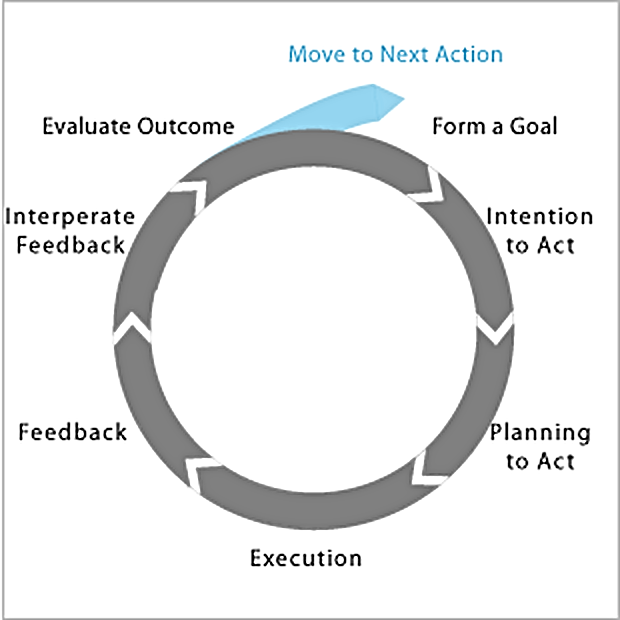
\includegraphics[width=0.4\textwidth]{grafiken/action_cycle.png}
 \caption{Human Action Cycle \cite{Kinser2011}}
 \label{fig:actionCycle}
\end{figure}
Um diesen Interaktionsverlauf zu gewährleisten und die Probleme zu minimieren, definierte Norman 6 Designprinzipien:
\begin{itemize}
	\item \textbf{Sichtbarkeit:} Wichtige Funktionen sollten für den Nutzer auf Anhieb sichtbar sein
	\item \textbf{Feedback:} Das System sollte nach einer Aktion sofort eine Rückmeldung geben
	\item \textbf{Einschränkungen:} Im aktuellen Zustand unzulässige Funktionen sollten ausgeblendet oder eindeutig erkennbar deaktiviert werden
	\item \textbf{Aktion und Wirkung:} Für jedes Interaktionselement sollte klar erkennbar sein, wie und worauf es sich auswirkt
	\item \textbf{Konsistenz:} Für identische Interaktionen sollten immer die gleichen Bedienelemente verwendet werden
	\item \textbf{Affordance:} Objekte sollten durch ihre Gestalt (Form, Farbe, etc.) eine Selbsterklärungsfähigkeit besitzen \cite{Ullenboom2014}
\end{itemize}
%%\subsubsection{Eingabegeräte} \label{sec:inputDevices}
%\heading{Maus}
%
%\heading{Tastatur}
%
%\heading{Touch}
\section{Visual Design} \label{sec:uid}
\textit{\enquote{Das Visual Design beschäftigt sich mit der Gestaltung einer Benutzeroberfläche \cite[S. 182]{Ullenboom2014}.}} Es baut auf den Beschlüssen in der Phase des Interaktionsdesign auf und verleiht der Oberfläche ihre finale Gestalt.\par
Der Visual Designer kümmert sich dabei um die Erstellung von prototypischen Designvorschlägen, die unter Anwendung von Designgrundlagen und -richtlinien entstehen. Das Ziel hierbei ist es, ein Konzept zu erstellen, das zugleich den Nutzer anspricht und zusätzlich die Usability durch Beachtung oben genannter Grundsätze verbessert. Im Laufe des Prozesses werden Objekte so platziert und gestaltet, dass eine einfache Orientierung möglich ist. Durch Farbkonzepte, basierend auf Erkenntnissen der Farbpsychologie, kann die Aufmerksamkeit konkret auf bestimmte Elemente gelenkt und Emotionen ausgelöst werden (durch Assoziation von Farben mit Elementen der Realität). Weitere Themengebiete sind Typographie, also das Auswählen von Schriftform, -größe, etc. und das Erstellen von Grafiken, Symbolen und Piktogrammen. \cite[S. 182]{Ullenboom2014}.

\subsection{Gestaltgesetze} \label{sec:uidRules}
Bei den Gestaltgesetzen handelt es sich um neuropsychologische Grundsätze, nach denen Objekte vom Menschen wahrgenommen und interpretiert werden. Berücksichtigt man diese Gesetze beim Design von Benutzeroberflächen, lassen sich Wahrnehmungseffekte auf subtile Weise erzeugen. Zum Beispiel kann die Aufmerksamkeit des Nutzers verstärkt auf gewisse UI-Elemente gelenkt oder die Bedienung vereinfacht werden. Nichtbeachtung dieser Regeln kann zu einer chaotisch wirkenden Benutzeroberfläche führen. Die wichtigsten Gestaltgesetze sind folgend aufgeführt.\par
\heading{Gesetz der Nähe}
\textit{\enquote{Objekte, welche nahe beieinander liegen, werden vom Auge gruppiert \cite[S. 186]{Moser2012}.}}\par
\begin{figure}[H]
 \centering
 
\includegraphics[width=0.25\textwidth]{grafiken/Gesetz_Naehe.png}
 \caption{Gesetz der Nähe \cite{Schossmann}}
 \label{fig:gesetzNaehe}
\end{figure} 
Durch Verringern der Abstände oder Vergrößern der Weißräume zwischen UI-Elementen, kann bewusst eine Gruppierung eingeführt werden, ohne dass zusätzliche Trennlinien oder Container von Nöten sind \cite[S. 186]{Moser2012}.\par
\heading{Gesetz der Ähnlichkeit}
\textit{\enquote{Visuell ähnliche Objekte werden vom Auge gruppiert \cite[S. 187]{Moser2012}.}}\par
\begin{figure}[H]
 \centering
 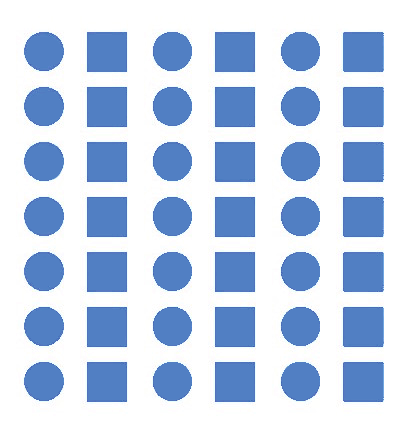
\includegraphics[width=0.25\textwidth]{grafiken/Gesetz_Aehnl.png}
 \caption{Gesetz der Ähnlichkeit \cite{Grigo}}
 \label{fig:gesetzAehnl}
\end{figure} 
Schaltflächen können auch durch Verwendung verschiedener Formen, Farben oder Größen voneinander abgegrenzt und gruppiert werden. Besonders bei der Visualisierung von Datenbeständen in Diagrammen (Farbe und Form der Datenpunkte und der Legende) ist diese Eigenschaft hilfreich \cite[S. 187]{Moser2012}.\par
\heading{Gesetz der Prägnanz}
\textit{\enquote{In einer Vielzahl von Objekten werden diejenigen zuerst wahrgenommen, welche sich durch ein oder mehrere Merkmale vom Rest abheben \cite[S. 187]{Moser2012}.}}\par
\begin{figure}[H]
 \centering
 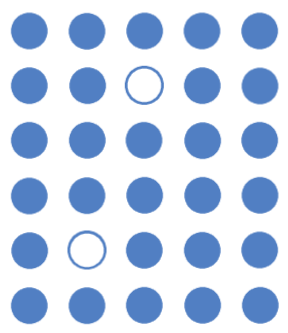
\includegraphics[width=0.25\textwidth]{grafiken/praegnanz.png}
 \caption{Gesetz der Prägnanz}
 \label{fig:gesetzPraeg}
\end{figure}
Ist ein Element oder eine Information \enquote{besonders} dargestellt, wird sie als erstes wahrgenommen. So können wichtige Informationen oder Bedienelemente hervorgehoben werden.\par
\heading{Gesetz der Kontinuität}
\textit{\enquote{Dieses Gesetz besagt, dass zum Beispiel Linien an Schnittpunkten eher als Fortführung ihrer bisherigen Linienführung, denn als eine Richtungsänderung gesehen werden \cite{Grigo}.}}\par
\begin{figure}[H]
 \centering
 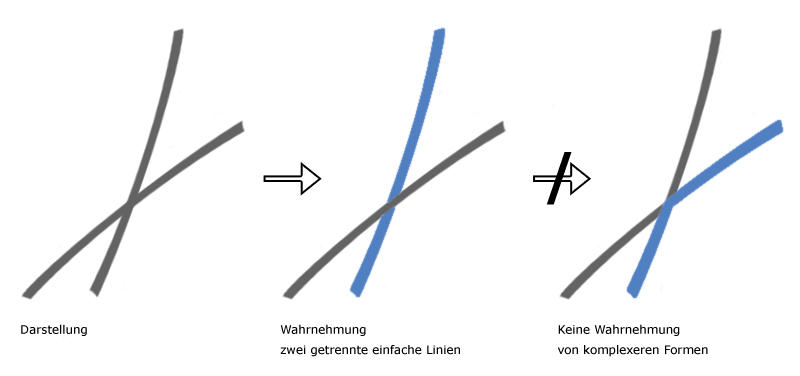
\includegraphics[width=0.8\textwidth]{grafiken/kontinuitaet.png}
 \caption{Gesetz der Kontinuität \cite{Grigo}}
 \label{fig:gesetzKonti}
\end{figure}
Elemente mit sanften Konturübergängen werden eher als Einheit erkannt als Elemente mit harten Übergängen \cite{Moser2012}.  Dies lässt sich unter anderem auf die Textorientierung anwenden. Sind mehrere Textzeilen nacheinander links orientiert, werden sie als zusammengehörig empfunden. Folgen daraufhin rechtsbündige Zeilen, bilden diese eine eigene Gruppe.\par
\heading{Gesetz der Geschlossenheit}
\textit{\enquote{Unser Auge komplettiert fehlende Teile einer Figur automatisch. \cite[S. 187]{Moser2012}.}}\par
\begin{figure}[H]
 \centering
 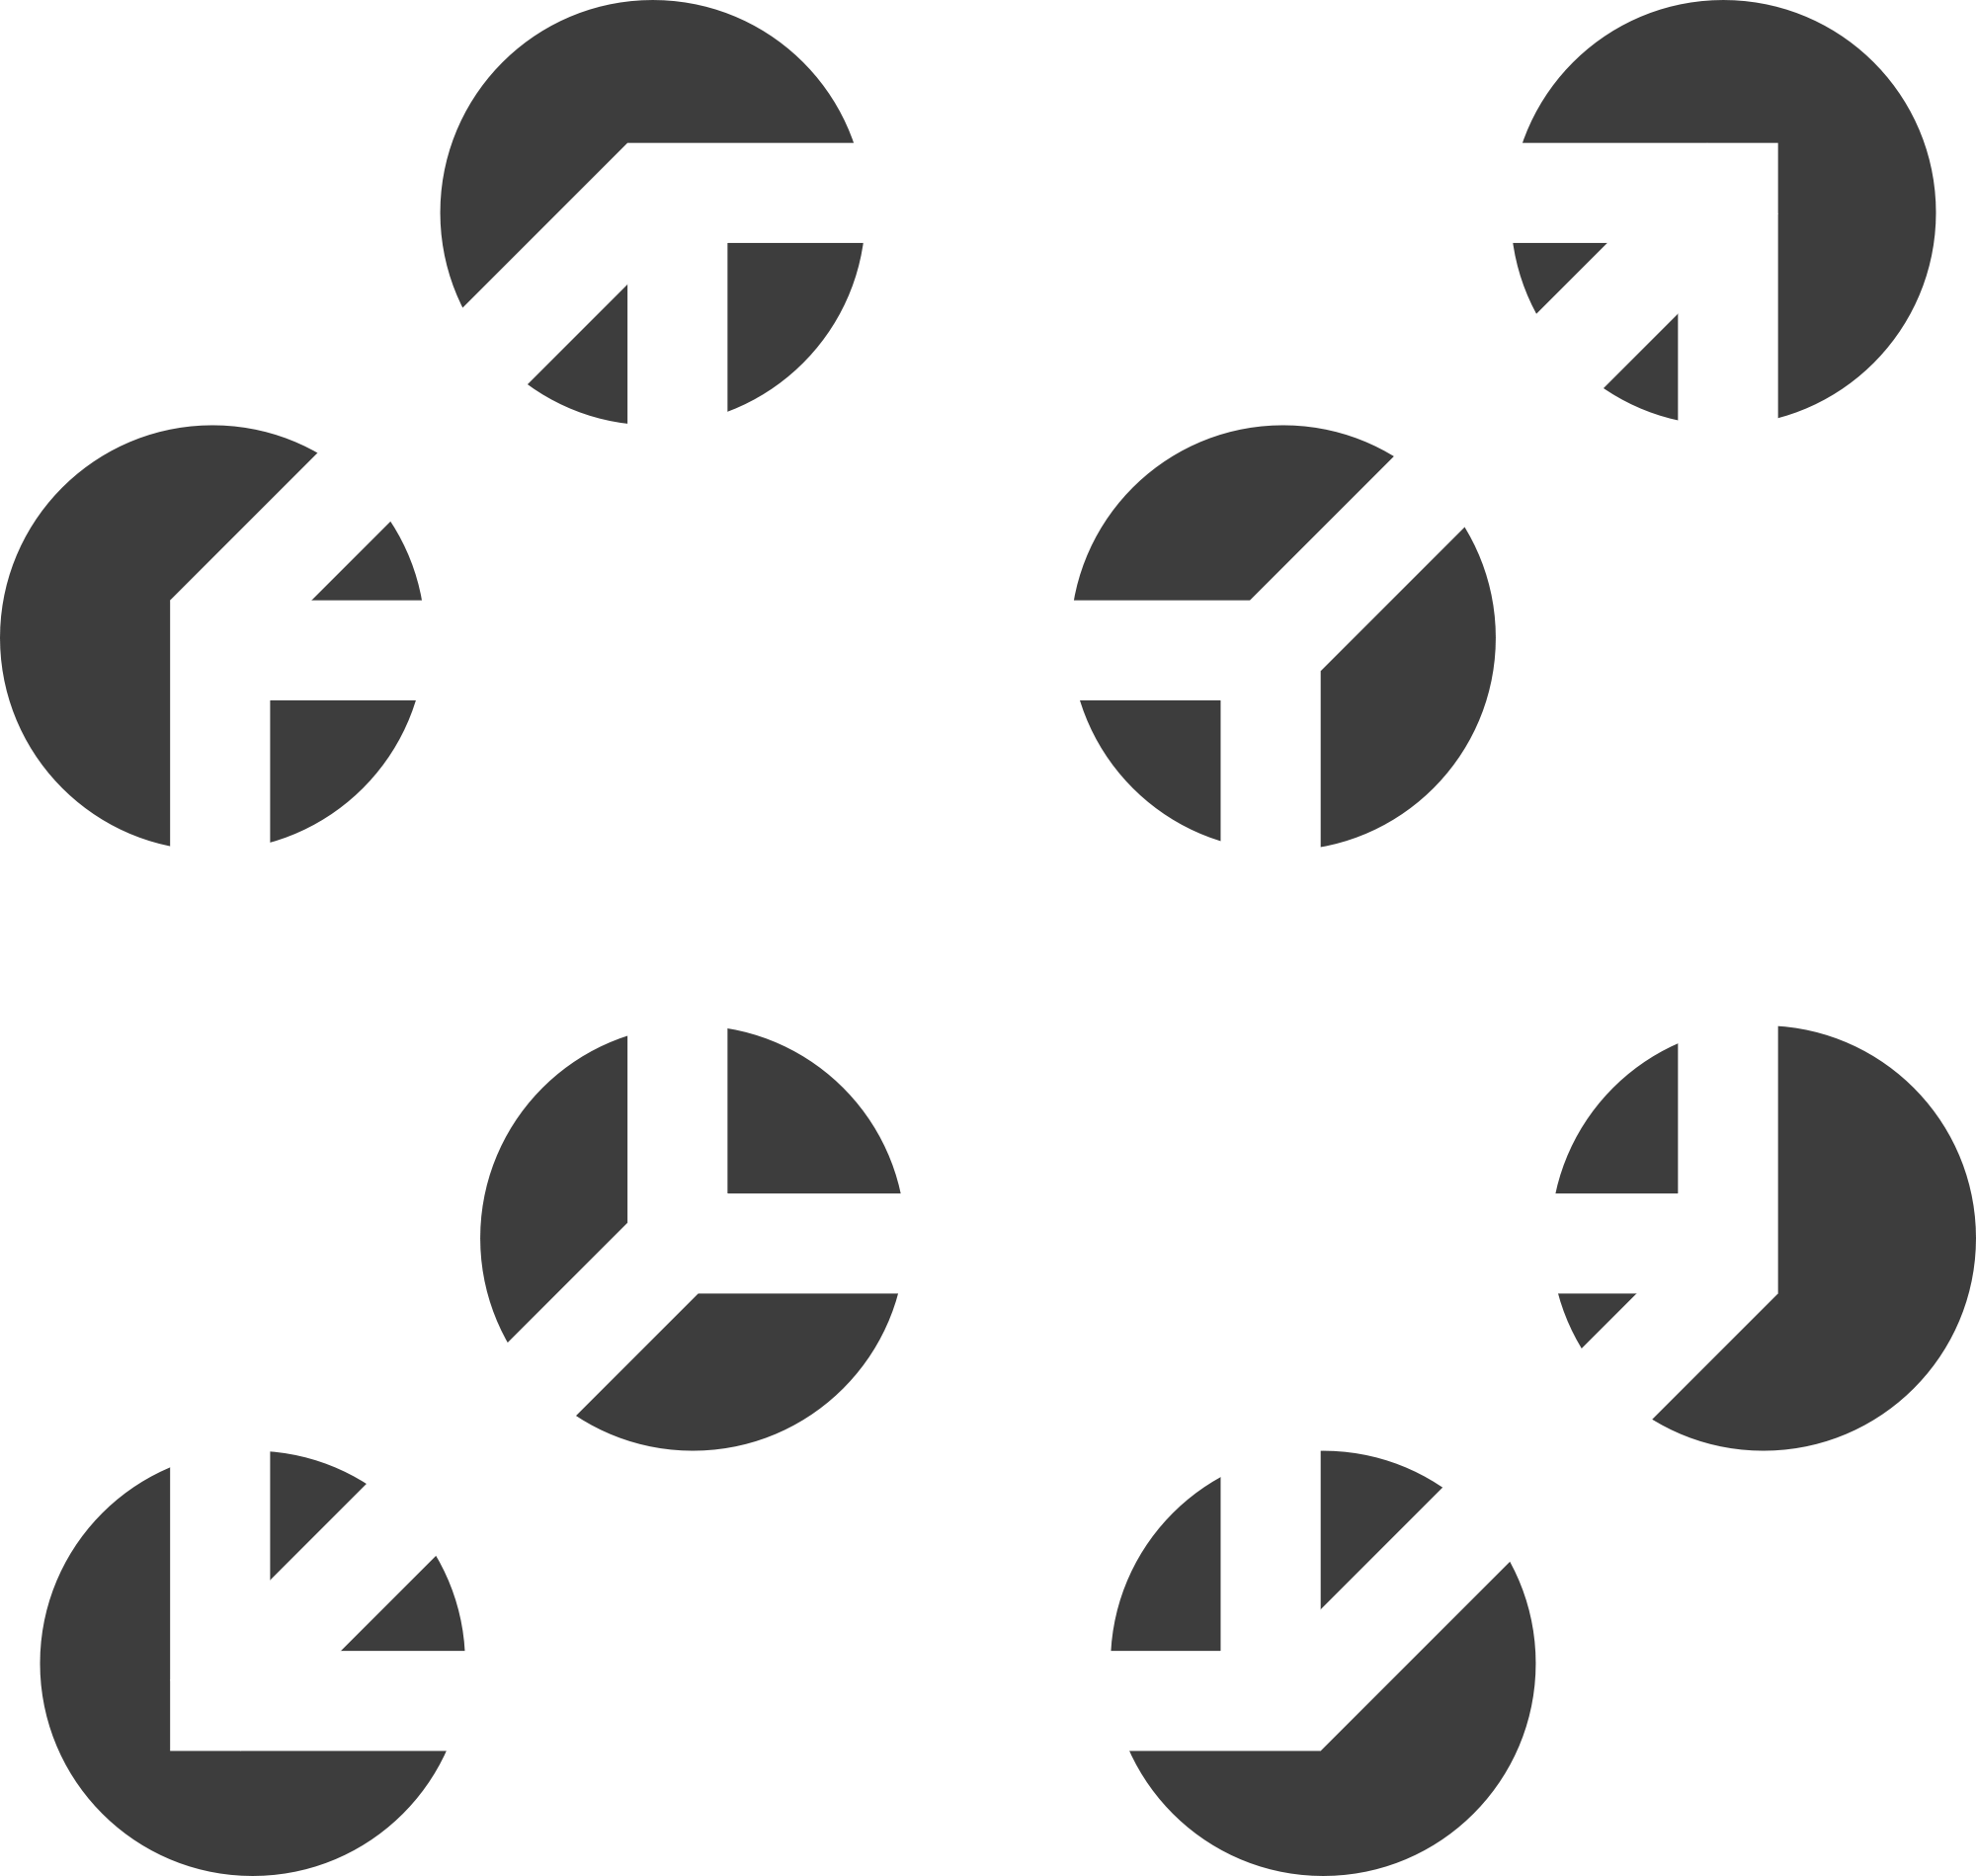
\includegraphics[width=0.25\textwidth]{grafiken/geschlossenheit.png}
 \caption{Gesetz der Geschlossenheit \cite{WikiGestaltgesetze}}
 \label{fig:gesetzGeschloss}
\end{figure}
Das Gesetz der Geschlossenheit kann dazu dienen, die Komplexität von Bedienelementen zu reduzieren, indem Teile davon weggelassen werden. Die fehlenden Bereiche werden durch die Wahrnehmung automatisch ergänzt. Dieser Effekt funktioniert jedoch nur bei dem Nutzer bekannten Formen \cite{Moser2012}.\par
\heading{Gesetz des gemeinsamen Schicksals}
\textit{\enquote{Wenn sich mehrere Objekte gleichzeitig oder in die gleiche Richtung bewegen, so werden sie als zusammengehörig empfunden \cite[S. 187]{Moser2012}.}}\par
\begin{figure}[H]
 \centering
 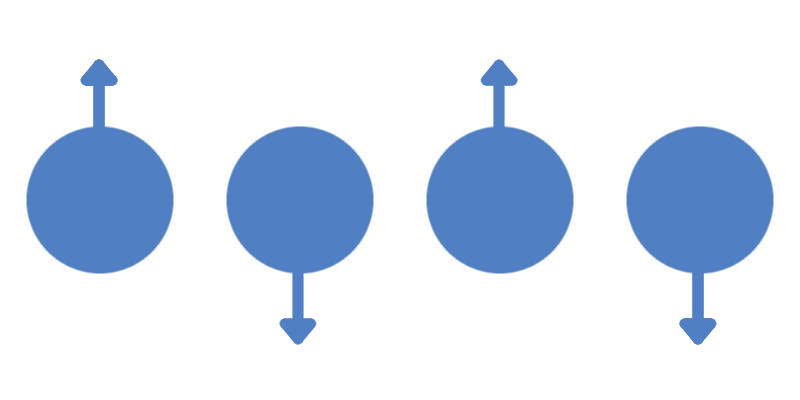
\includegraphics[width=0.2999\textwidth]{grafiken/schicksal.png}
 \caption{Gesetz des gemeinsamen Schicksals}
 \label{fig:gesetzSchicksal}
\end{figure}
Durch gleichzeitige bzw. gleichgerichtete Animation kann die Zusammengehörigkeit von Objekten erklärt werden \cite{Moser2012}. Unterschiedliche Animationen zur gleichen Zeit können dazu genutzt werden, die Unabhängigkeit verschiedener Gruppen zu betonen. In Abbildung \ref{fig:gesetzSchicksal} bspw. werden die sich nach oben und die sich nach unten bewegenden Elemente jeweils als eine Gruppe wahrgenommen.
\heading{Gesetz der gemeinsamen Region}
\textit{\enquote{Elemente in abgegrenzten Gebieten werden als zusammengehörig empfunden \cite{WikiGestaltgesetze}.}}\par
\begin{figure}[H]
 \centering
 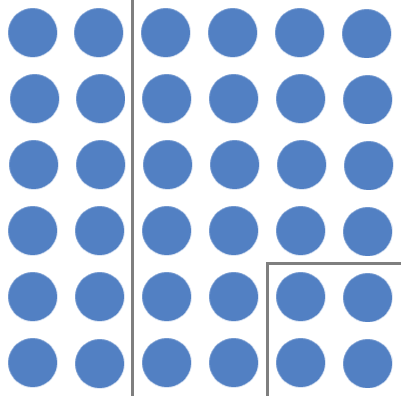
\includegraphics[width=0.25\textwidth]{grafiken/region.png}
 \caption{Gesetz der gemeinsamen Region}
 \label{fig:gesetzRegion}
\end{figure}
Die wohl trivialste Abgrenzung von Elementen kann durch die Benutzung von klassischen Trennlinien erfolgen. So werden die Objekte in mehrere Bereiche eingeteilt und innerhalb dieser Bereiche als zusammengehörig empfunden. Auch verschiedene Hintergrundfarben von Regionen führen zum gewünschten Effekt.

\subsection{DIN EN ISO 9241-110} \label{sec:uidNorms}
Sowohl im deutschen als auch internationalen Raum, gibt es seit geraumer Zeit Normen, die Grundsätze dafür liefern, wie Anwendungen gestaltet sein sollten. Für die Mensch-Computer-Interaktion ist insbesondere die \textit{DIN EN ISO 9241} von Bedeutung. In dieser sind Anforderungen an die Gestaltung von Hardware und Software, sowie das Arbeitsumfeld definiert. Besonders wichtig für das Thema User-Experience ist der Abschnitt 110. Dieser Abschnitt mit dem Titel \textit{Grundsätze der Dialoggestaltung} \enquote{behandelt die ergonomische Gestaltung von interaktiven Systemen und beschreibt Grundsätze der Dialoggestaltung, die grundsätzlich unabhängig von einer bestimmten Dialogtechnik sind, und die bei der Analyse, Gestaltung und Bewertung von interaktiven Systemen angewendet werden sollten \cite[S. 4]{DIN2006}.} Er wurde 2006 verfasst und ersetzt seitdem den vorherigen Teil 10 \cite{DIN2006}.\par
Um häufig auftretende Nutzungsprobleme zu vermeiden, definiert die Norm sieben Kriterien, nach denen die Gebrauchstauglichkeit einer Anwendung bewertet werden kann:
\begin{itemize}
	\item Aufgabenangemessenheit
	\item Selbstbeschreibungsfähigkeit
	\item Erwartungskonformität
	\item Lernförderlichkeit
	\item Steuerbarkeit
	\item Fehlertoleranz
	\item Individualisierbarkeit \cite[S. 7]{DIN2006}
\end{itemize}
Diese Kriterien überschneiden sich in einigen Punkten mit den von Nielsen definierten Kernaspekten der Usability, führen aber ergänzend die Selbstbeschreibungsfähigkeit, Steuerbarkeit und Individualisierbarkeit an.\par
Ein Dialog ist selbstbeschreibungsfähig, wenn ein Nutzer zu jeder Zeit feststellen kann, an welcher Stelle im Dialog er sich befindet, weiß, wie und wohin er von dort navigieren kann und welche Aktionen in der aktuellen Ansicht möglich sind \cite[S. 10]{DIN2006}. Die Steuerbarkeit beschreibt die Adaptivität des Dialogs an die Fähigkeiten und das Navigationsverhalten des Anwenders. Die Geschwindigkeit in der ein Nutzer Aktionen auf der Oberfläche durchführt, sollte möglichst allein durch den Nutzer bestimmt werden. Weiterhin sollte die Navigation den Nutzer nicht einschränken, sondern ihre Möglichkeiten aufzeigen und eine freie Navigation unterstützen \cite[S.13]{DIN2006}. Ein individualisierbarer Dialog ermöglicht es, die Informationsdarstellung in einem gewissen Rahmen an die Bedürfnisse des Anwenders anzupassen \cite[S.15]{DIN2006}. \par
Es ist nicht immer möglich, alle Grundsätze zu erfüllen. Stattdessen muss von Anwendung zu Anwendung gewichtet werden, auf welchen Aspekten der Schwerpunkt liegt. Beschränkende Faktoren können auf der einen Seite Budget- oder Zeitmangel sein, auf der anderen Seite können sich die Kriterien aber auch gegenseitig einschränken. Beispielsweise ist es schwerer möglich, eine gute Steuerbarkeit zu erreichen, wenn die Applikation hochindividualisierbar sein soll \cite{DIN2006}. Daher muss für eine gute Usability abgewägt werden, worauf bei der Umsetzung der Fokus gelegt werden soll.

\section{Usability-Evaluationsverfahren} \label{sec:methods}
Es gibt verschiedene Verfahrensweisen, die mit unterschiedlich viel Aufwand Aufschluss über die Gebrauchstauglichkeit einer Anwendung geben können. \enquote{Sie alle versuchen, durch unterschiedliche Ansätze, eine Aussage darüber zu treffen, wie effizient, effektiv und zufriedenstellend das Produkt von einem Benutzer verwendet werden kann. Jede Methode hat ihre eigenen Vor- und Nachteile \cite[S. 224]{Ullenboom2014}.}\par
Die Evaluationsmethoden können in zwei Arten unterteilt werden. Zum einen gibt es die analytischen Nutzertests, für die eine Gruppe an Testpersonen ausgewählt wird, die daraufhin Fragen beantworten oder Aufgaben mit dem Testsystem durchführen müssen. Die andere Art von Tests sind die die empirischen Expertentests. Für diese Analysen werden keine Testpersonen benötigt. Stattdessen wird anhand objektiver Kriterien und Verfahren versucht, die Effektivität, Effizienz und Nutzerzufriedenheit zu erhöhen. Für die Auswahl der zu verwenden Testmethoden müssen sowohl die Anforderungen an diese, als auch die Güte der Methoden in Betracht gezogen werden. Je nach Art des Testes stellt dieser Ansprüche an das Fachwissen des Testers und den nötigen Aufwand um die Tests durchzuführen. Der Nutzen eines Tests setzt sich aus seiner Objektvität, seiner Zuverlässigkeit und seiner Gültigkeit zusammen \cite[S.224 f.]{Ullenboom2014}.\par
Der Ablauf eines gesamten Testvorganges ist nach Ullenboom folgender:
\begin{enumerate}
	\item \textbf{Ziel und Zweck festlegen:} Es muss festgelegt werden, was der Untersuchungsgegenstand ist und was der Zweck der Untersuchung ist
	\item \textbf{Untersuchungsdesign entwerfen:} Bei dem Entwurf müssen Faktoren wie Zeit, Ressourcen und Stand des Projektes mit einbezogen werden
	\item \textbf{Teilnehmer rekrutieren:} Bei Nutzertests müssen Teilnehmer ausgewählt werden, die nach Möglichkeit verschiedene Anwendertypen repräsentieren.
	\item \textbf{Evaluation vorbereiten:} Das Szenario, das getestet werden soll, muss vorbereitet und die entsprechende Testumgebung geschaffen werden.
	\item \textbf{Evaluation durchführen} Die Tests werden durchgeführt. Währenddessen wird das Verhalten der Nutzer dokumentiert. Dies beinhaltet unter Anderem, wie zielgerichtet der Anwender die gegebenen Aufgaben lösen kann.
	\item \textbf{Resultate auswerten:} Anhand der dokumentierten Daten können nun Problemstellen identifiziert und ausgebessert werden. Dazu erfolgt im Team eine Gewichtung der Probleme und wenn möglich die Aufnahme erster Lösungsansätze.
\end{enumerate}
Für die Durchführung der Nutzertests ist nach Nielsen eine Probandengruppe von 5 Personen völlig ausreichend. Studien zufolge entdeckt ein einzelner Testanwender rund 31\% der Usability-Probleme einer Anwendung \cite{Nielsen2000}. Testet man mit mehreren Nutzern, findet jeder dieser Nutzer im Mittel 31\% der vorhandenen Fehler. Dabei werden zum Teil neue Probleme ans Licht gebracht, aber auch bereits bekannte wiederholt entdeckt. Forschungen haben ergeben, dass der Anteil gefundener Usability-Probleme aus diesem Grund wie folgt berechnet werden kann:
\begin{equation}
			1-(1-L)^n\text{ \cite{Nielsen2000}}
\end{equation}
Dabei ist \(n\) die Anzahl an Testpersonen und \(L\) der Anteil gefundener Usability-Probleme pro Testsubjekt (31\%) \cite{Nielsen2000}. Das bedeutet bei 5 Testpersonen eine Abdeckung von rund 85\%. Das Testen mit mehr Anwendern würde das Budget stark belasten und wenig zusätzlichen Nutzen mit sich bringen. Daher ist es sinnvoller, in vielen Durchläufen mit wenigen Personen zu testen, als in wenigen Durchläufen mit vielen \cite{Nielsen2000}.\par
\heading{Hallway-Testing}
Das Hallway-Testing ist eine sehr informelle Methode, erstes Feedback über die Usability eines kleinen Programmteiles zu erhalten. Das Prinzip des Hallway-Testing ist es, einen beliebigen zu fragen, was er von einer bestimmten Funktion hält. Dazu wird eine kurze Aufgabe gestellt (wie z.B. \enquote{Drucke dieses Dokument}) und beobachtet, wie der Kandidat sich verhält. Bei komplexeren Sachverhalten wird so kurz wie möglich die Fachlichkeit bzw. der Nutzungskontext erklärt. Ohne Hinweise für die Lösung zu geben, wird die Aufgabe kurz erklärt. Bei der Durchführung denkt der Testnutzer laut mit \cite[S. 226]{Ullenboom2014}.
Mit sehr wenig Aufwand können durch diese Methode während der Entwicklung grobe Nutzungsprobleme beseitigt werden.\par
\heading{Pluralistic Walkthrough}
Beim Pluralistic Walkthrough handelt e sich um eine Art von Nutzertests. Die Testkandidaten werden in einer Art Workshop versammelt und bekommen die Anwendung grob vorgestellst, sodass sie sich auf dem Wissensstand eines durchschnittlichen Erstbenutzers befinden. Daraufhin wird die Aufgabenstellung unterbreitet und die Nutzer versuchen diese mit der ihnen gegebenen Anwendung umzusetzen. Am Ende des Tests wird die Optimallösung vorgestellt. Die Testanwender beschreiben daraufhin ihre Lösung. Zum Feststellen der konkreten Usability-Probleme, also der Gründe, warum eine andere Lösung gewählt oder gefunden wurde, wird zum Abschluss über die Lösungen diskutiert und die Fehlerquellen herausgearbeitet \cite[S. 228]{Ullenboom2014}.\par
\heading{Formaler Usability-Test}
Bei dieser Methode werden Testpersonen einzeln mit der Bedienung eines Programmes betraut. Nachdem festgelegt wurde, welche Teile der Anwendung getestet werden sollen, werden Aufgaben formuliert und niedergeschrieben. Diese Aufgaben erhält der Testkandidat in schriftlicher Form. Er versucht diese mit der vorliegenden Anwendung zu lösen und wird währenddessen beobachtet. Zu diesem Zweck wird zum Einen der Bildschirminhalt aufgezeichnet und zum anderen die Reaktion des Teilnehmers selbst analysiert \cite[S. 230]{Ullenboom2014}.\par
Der Test muss sorgsam vorbereitet werden. Dazu gehört sowohl die Installation der zu testenden Software, als auch das Aufsetzen des Aufnahmemoduls, dass die Interaktion und ggf. den Nutzer selbst aufzeichnet. Um die Aufgabenstellungen lösen zu können, sind ggf. Testdaten erforderlich, die erst noch eingespielt werden müssen. Auch darf nicht vergessen werden, das System zurückzusetzen, nachdem ein Testnutzer Änderungen daran gemacht hat. \cite[S.231]{Ullenboom2014}\par
Während der Instruktion des Nutzers wird dieser gebeten, während des Tests laut mitzudenken. Diese Technik wird \textbf{\textit{Thinking Aloud}} genannt. Dies hilft dabei, die Absichten, Gefühle und Eindrücke des Anwenders zu ergründen \cite[S. 1]{Fromman2005}. Nach Start des Tests wird durch das Testpersonal keine Hilfestellung mehr gegeben. Weiß der Nutzer nicht, wie er weiter zu verfahren hat, wird der Testdurchlauf abgebrochen \cite[S. 231]{Ullenboom2014}.
\heading{Heuristische Evaluation}
Die Heuristische Evaluation ist ein beliebtes Expertentestverfahren. Der Tester untersucht im Rahmen dieser Methode eine Anwendung auf Basis von Heuristiken. In der Regel werden mehrere Usability-Experten eingesetzt, um die Erkennungsrate von Problemen zu erhöhen. Am Ende werden die Ergebnisse zusammengetragen und für jedes gefundene Problem ein Schweregrad ermittelt. Dieser setzt sich aus den Faktoren \textit{Auftretenswahrschienlichkeit}, \textit{Grad der Beeinflussung} und \textit{der Möglichkeit, das Problem zu umgehen}, zusammen. Da die definierten Heuristiken eine gewisse Sicherheit bieten, kann diese Methode auch von weniger erfahrenen Testern angewandt werden \cite[S. 232f.]{Ullenboom2014}.\par
\heading{Cognitive Walkthrough}
Der Expertentest \enquote{Cognitive Walkthrough} ist ein Verfahren, bei dem der Usability-Tester versucht, sich in die Lage des Anwenders zu versetzen und die Anwendung zu bedienen. Um dies adäquat tun zu können, müssen zunächst die genauen Arbeitsabläufe der Endanwender erschlossen werden. Hierbei ist es sinnvoll, verstärkt komplexe Arbeitsabläufe zu testen \cite[S. 234]{Ullenboom2014}.\par
Der erste Schritt der Analyse ist die \textit{Definition des Inputs}. Nach Ullenboom sind dazu folgende Schritte notwendig:
\begin{enumerate}
	\item Festlegen, welcher Teil getestet werden soll
	\item Verstehen der Arbeitsabläufe
	\item Formulieren von praxisnahen Aufgaben
	\item Wahl einer geeigneten Benutzerrolle
	\item Vorbereiten eines Prototypen \cite[S. 234]{Ullenboom2014}
\end{enumerate}
Bei der Durchführung werden die Aufgaben anhand des Prototypens versucht umzusetzen. Dabei wird davon ausgegangen, dass der Nutzer stets versucht, den Weg zu nehmen, den er für den einfachsten hält. Es muss bei jeder Aktion geprüft werden, ob während der Interaktion die folgenden Fragen geklärt werden:
\begin{itemize}
	\item Wird der Benutzer versuchen, den richtigen Effekt zu erzielen?
	\item Wird der Benutzer erkennen, dass die korrekte Aktion zur Verfügung steht?
	\item Wird der Benutzer eine Verbindung zwischen der korrekten Aktion und dem gewünschten Effekt herstellen?
	\item Wenn die korrekte Aktion ausgeführt wurde: Wird der Benutzer den Fortschritt erkennen? \cite[S. 234]{Ullenboom2014}
\end{itemize}
Wenn sich bei einer dieser Fragestellungen Probleme zeigen, müssen diese unter Angabe des entsprechenden Handlungsschrittes, dem Grund der Probleme und möglicher Verbesserungsvorschläge dokumentiert werden. Aufgrund dieser Aufzeichnungen kann die Benutzerschnittstelle überarbeitet werden.\par
\heading{Usability-Befragung}
\enquote{Die Usability-Befragung ist eine quantitative Methode, bei der die Usability mit Hilfe eines Fragebogens ermittelt wird \cite[S. 236]{Ullenboom2014}.} Es ist eine Art von Nutzertest, die darauf abzielt, einen möglichst großen Anwenderbereich abzudecken. Für die Auswahl des Fragebogens gibt es mehrere Möglichkeiten:
\begin{enumerate}
	\item \textbf{Standardisierter Fragebogen:} Es gibt eine Reihe standardisierter Fragebögen, mit deren Hilfe ein Grobüberblick über verschiedene Aspekte der Usability einer Anwendung erlangt werden kann.
	\item \textbf{Teilstandardisierter Fragebogen:} Verwendung von standardisierten Fragebögen, angepasst an die zu evaluierende Anwendung (z.B. Freitextfelder für weitergehende Informationen)
	\item Selbstentwickelter Fragebogen: Durch die Entwicklung eines speziell auf die Anwendung zugeschnittenen Fragebogens können die exaktesten Ergebnisse erzielt und konkrete Problemstellen identifiziert werden. Dies erfordert allerdings einigen Aufwand und entsprechendes Know-How.
\end{enumerate}
\heading{KLM/GOMS}
\textit{GOMS} ist eine Methode zur Evaluation der Effizienz eines Softwaresystems. Durch das Anwenden gewisser Regeln ist es möglich, die Zeitdauer abzuschätzen, die für eine Interaktion benötigt wird. Dazu ist es zuerst von Nöten, alle Schritte der Interaktion zu identifizieren. Diese Schritte werden in atomare Aktivitäten zerlegt, deren einzelne durchschnittliche Dauer durch empirische Analysen ermittelt wurde.\par
GOMS steht für \textit{Goals, Operators, Methods and Selection Rules}. Dies ist gleichzeitig das Modell, das der Interaktion eines Benutzers zugrunde liegt:
\begin{itemize}
	\item \textbf{Ziele:} Die Ziele, die der Benutzer erreichen möchte (Bsp. Dokument drucken)
	\item \textbf{Operatoren:} Die atomaren Handlungsschritte (Bsp. Drücken einer Taste, Warten auf Feedback der Software)
	\item \textbf{Methoden:} Kombination von Operatoren zu einer Interaktion, die den Nutzer an sein Ziel bringt
	\item \textbf{Selektionsregeln:} Nach diesen Regeln entscheidet der Benutzer, welche mögliche Methode er einsetzt
\end{itemize}
KLM-GOMS ist eine spezielle, einfache Variante des GOMS-Modells. Es verwendet nur sechs Operatoren, die die atomaren Handlungsschritte darstellen:
\begin{table}[h!]
 \centering
 \begin{tabular}{|l|c|r|} \hline
 \textbf{Aktion} & \textbf{Code} & \textbf{Dauer} \\ \hline
 Tastendruck & K & \specialcell{Profi Schreiber:&\myTab 0.08 s\\Guter Schreiber:&\myTab 0.20 s\\Anfänger:&\myTab 1.20 s\\Zufällige Buchst.:&\myTab 0.50 s\\Codes:&\myTab 0.75 s} \\ \hline
 Maus positionieren & P & 1.1 s \\ \hline
 Tastatur-/Maus- Wechsel & H & 0.4 s \\ \hline
 Maustaste & B & 0.1 s \\ \hline
 Kurz überlegen & M & 1.2 s \\ \hline
 Antwortzeit & W(t) & Unterschiedlich (je nach t) \\ \hline
 \end{tabular}
 \caption{KLM Zeitwerttabelle}
 \label{tab:klm}
\end{table}
\heading{A/B-Test}
A/B-Tests dienen dazu, zwei verschiedene Produkte oder Lösungsvarianten miteinander zu vergleichen. Dies geschieht in der Regel in Form von Nutzertests. Dabei bedienen zwei Nutzergruppen gleichzeitig die verschiedenen Systeme und versuchen eine gestellte Aufgabe zu lösen. Dazu wird ein Kriterium definiert, anhand dessen bestimmt werden kann, ob die Interaktion erfolgreich war (z.B. Operationen so gewählt wie durch das Design vorgesehen). Die Lösung, bei der die Testnutzer quantitativ erfolgreicher waren, ist die Alternative mit der besseren Usability \cite[S. 240]{Ullenboom2014}.\par
Zum Vergleich der Effizienz zweier Anwendung wird häufig eine GOMS-Analyse der beiden Software-Produkte durchgeführt. Dies muss mit vergleichbaren Aufgabenstellungen geschehen, damit die Ergebnisse repräsentativ sind.\par
\heading{Eyetracking}
Eytracking ist eine ergänzende Methode, die die Aussagefähigkeit eines Nutzertests erhöhen kann. Es zielt speziell darauf ab, zu erkennen, welchen Bereichen der Anwender vermehrt Aufmerksamkeit schenkt und welche er gar nicht beachtet \cite{Henrici2010}.\par
Es gibt verschiedene technische Lösungen, um Eyetracking umzusetzen. Eine davon ist die Benutzung einer Eyetracking-Kamera, die zusätzlich zu einem Monitor aufgestellt werden kann. Das Modul besteht aus einer Kameralinse und einer Infrarot-Lichtquelle. Das für das menschliche Auge unsichtbare Infrarot-Licht erzeugt auf der Hornhaut eine sogenannte \enquote{korneale Reflexion}. Diese Reflexion befindet sich immer über, unter oder neben der Pupille. die Pupille selbst reflektiert das Licht nicht. Aus der relativen Position der Reflexion zur Pupille kann nach geeigneter Kalibrierung der Blickpunkt auf dem Bildschirm errechnet werden.\par
\begin{figure}[H]
 \centering
 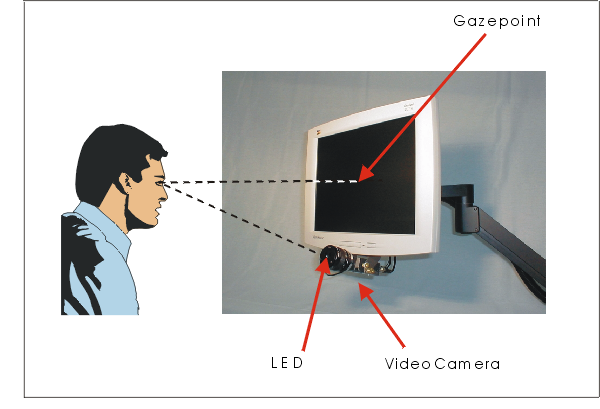
\includegraphics[width=0.45\textwidth]{grafiken/eyegaze.png}
 \caption{Eyetracking \cite{Eyegaze}}
 \label{fig:eyetracking}
\end{figure}
Während der Aufzeichnung können typischerweise zwei wesentliche Arten von Daten gesammelt werden, die mit der Blickrichtung zusammen hängen. Dies sind die Fixation und die Sakkade. Unter Fixation wird der Fokussierung der Augen auf einen bestimmten Bildpunkt verstanden. Dazu gehört die Position und die Dauer der Fokussierung. Eine Sakkade ist der Sprung von einer Fixation zur nächsten. Dies geschieht extrem schnell, sodass zu dieser Zeit mit herkömmlichen Eyetracking-Systemen keine verwertbaren Daten gemessen werden können. Zusätzlich zu diesen Informationen lässt sich auch die Pupillengröße ermitteln. Diese Daten sind allerdings im Rahmen der Usability-Tests kaum von Relevanz.\par
Die gesammelten Daten lassen sich nun auf mehrere Arten und Weisen visualisieren \cite{Henrici2010}.\par
Heatmaps und Gaze-Opacity Visualisierungen  zeigen mithilfe von Farbcodes, auf welchen Elementen bzw. Bereichen Fixationen erkannt wurden und wie lange diese gedauert haben. Dabei stehen warme Farben meist für längere Fixationen. Parallel dazu lässt sich eine Gaze Opacity Grafik erstellen, die Bereiche schwarz einfärbt, wenn diese kaum oder gar nicht wahrgenommen wurden \cite{Henrici2010}.
\begin{figure}[H]
 \centering
 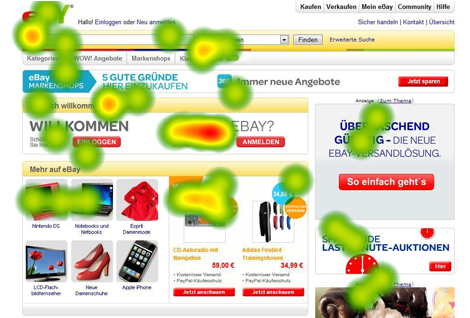
\includegraphics[width=0.48\textwidth]{grafiken/heatmap.png}
 \caption{Beispiel Heatmap \cite{Henrici2010}}
 \label{fig:heatmap}
\end{figure}
\begin{figure}[H]
 \centering
 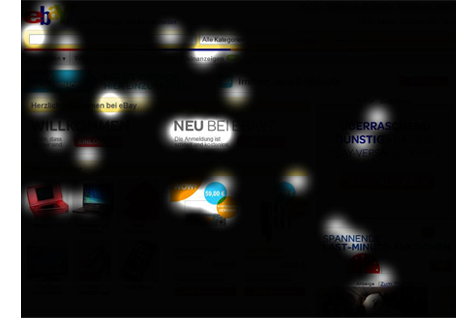
\includegraphics[width=0.48\textwidth]{grafiken/gaze_opacity.png}
 \caption{Beispiel Gaze Opacity \cite{Henrici2010}}
 \label{fig:gazeOpacity}
\end{figure}
Bei der Areas of Interest wird die Oberfläche in verschiedene Bereiche eingeteilt. Die Fixationen in den einzelnen Bereichen werden zusammengezählt und der prozentuale Anteil hinsichtlich der Gesamtheit der Fixationen (und ihrer Dauer) während des gesamten Tests ermittelt. Jedem Bereich kann eine Farbe zugewiesen werden, die als Schlüssel zu der in der Legende festgehaltenen Prozentzahl dient.
\begin{figure}[H]
 \centering
 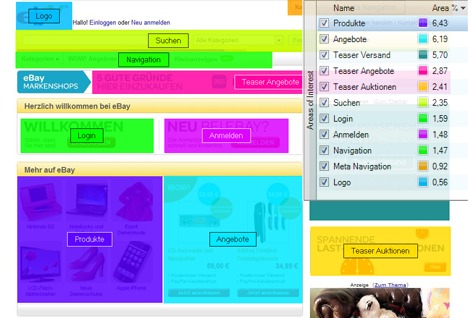
\includegraphics[width=0.48\textwidth]{grafiken/areas_of_interest.png}
 \caption{Beispiel Areas of Interest \cite{Henrici2010}}
 \label{fig:areasOfInterest}
\end{figure}
Die letzte Visualisierung beachtet zusätzlich die Reihenfolge der Fixationen. Es werden verschieden große Kreise genutzt, um Fixationen unterschiedlicher Dauer darzustellen. Diese werden in der richtigen Reihenfolge durch Linien verbunden, welche die synthetisierten Sakkaden darstellen.
\begin{figure}[H]
 \centering
 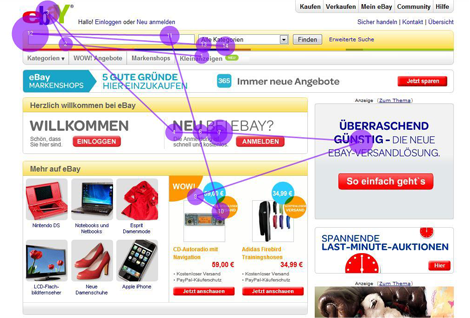
\includegraphics[width=0.48\textwidth]{grafiken/gaze_plot.png}
 \caption{Beispiel Gaze Plot \cite{Henrici2010}}
 \label{fig:gazePlot}
\end{figure}
\heading{Bewertung der Testverfahren}
Die Testverfahren können nach verschiedenen Kriterien bewertet werden. Ein Teil der Kriterien betrachtet die Anforderungen an das Budget und den Tester, der andere Teil beschäftigt sich mit der Qualität der Ergebnisse. Optimal sind Tests, wenn sie möglichst geringe Anforderungen haben, aber aussagekräftige Ergebnisse liefern. Ein Faktor, der in dieser Übersicht nicht bedacht ist, ist der Zeitpunkt, zu dem die Tests durchgeführt werden können. Das Hallway Testing kann bspw. nur während einer laufenden Entwicklung an einer Komponente durchgeführt werden und eignet sich nicht als Testmethode für ein, möglicherweise komplexes, fertiges System.
\begin{table}[h!]
		\begin{tabular}{|l|c|c|c|c|c|c|}
			\hline
			\textbf{Methode}&\textbf{Fachwis.}&\textbf{Aufwand}&\textbf{Effektiv.}&\textbf{Validität}&\textbf{Zuverl.}&\textbf{Objektiv.}\\
			\hline
			\twolinecell{Hallway\\Testing} & \star & \star & \star \star & \star & \star & \star\\
			\hline
			\twolinecell{Usability\\Walkthrough} & \star \star & \star \star & \star \star & \star \star & \star & \star\\
			\hline
			\twolinecell{Formaler\\Usability-Test} & \star \star & \star \star \star & \star \star \star & \star \star \star & \star \star & \star \star\\
			\hline								
			\twolinecell{A/B-Test\\[2.3ex]} & \star \star & \star \star & \star \star & \star \star \star & \star \star & \star \star \star\\
			\hline
			\twolinecell{Heuristische\\Evaluation} & \star \star \star & \star & \star \star \star & \star \star & \star \star \star & \star\\
			\hline
			\twolinecell{Usability-\\Befragung} & \star & \star & \star & \star \star & \star \star & \star \star \star\\
			\hline
			\twolinecell{GOMS\\[2.3ex]} & \star \star & \star \star & \star & \star \star & \star \star \star & \star \star \star\\
			\hline
		\end{tabular}
		\caption{Gütekriterien von Evaluationsmethoden nach Ullenboom \cite[S. 225]{Ullenboom2014}}
	\label{tab:hallwayTesting}
\end{table}
\section{JavaFX} \label{sec:javaFX}
JavaFX ist das aktuellste GUI-Framework der Java-Plattform. Es wird standardmäßig mit Java SE 8 ausgeliefert und soll den Vorgänger \textit{Swing} ersetzen \cite{Mueller2015}.\par
Die neuartige Technologie vereinigt verschiedene Konzepte, die den Entwickler bei der Entwicklung einer Benutzeroberfläche unterstützen.
\begin{itemize}
	\item \textbf{\textit{Szenegraph}:} Sämtliche Bedienelemente sind in einer Baumstruktur, ausgehend von einem Wurzelknoten, angeordnet.
	\item \textbf{Styling:} Das Aussehen aller UI-Komponenten kann mit Hilfe von CSS-Dateien angepasst werden.
	\item \textbf{Animationen:} Es können auf unkomplizierte Weise Animationen erstellt und auf beliebige angezeigte Objekte angewandt werden.
	\item \textbf{FXML:} Die Struktur der Oberfläche kann sowohl in Java-Code, als auch in XML-basierten Dateien, sogenannten FXML-Dateien, definiert werden.
	\item \textbf{Properties und Bindings:} Alle Controls haben gewisse Eigenschaften (Properties), die sich dynamisch verändern lassen. So kann man ein Property an ein gleichartiges binden. Verändert sich der Wert der einen Eigenschaft, wird der Wert der anderen ebenfalls geändert.
\end{itemize}
\subsection{Eventhandling} \label{sec:javafxEventhandling}
Besonders relevant für die Arbeit ist das Konzept des Eventhandlings in JavaFX.\par
Ein Event ist eine Eingabe, die durch den Nutzer getätigt wurde. Dies kann z.B. das Drücken oder Loslassen einer Taste auf der Tastatur sein. Auch das Klicken auf ein Bedienelement und das Ausführen einer Geste auf einem Touchscreen stellen Events dar. Jedes dieser Events kann an bestimmten Stellen im Code behandelt werden.\par
Wie in Abschnitt \ref{sec:javaFX} bereits erwähnt, ist die Komponentenstruktur in JavaFX baumartig aufgebaut. Der Wurzelknoten im Szenegraphen ist die \textit{Stage}. Diese entspricht dem sichtbaren Fenster, in dem die Anwendung läuft. Sie hat als einziges Kind die \textit{Scene}, die alle weiteren Elemente enthält.
\begin{figure}[H]
 \centering
 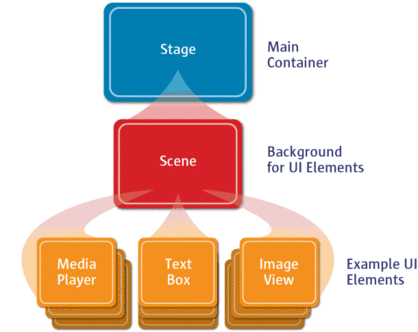
\includegraphics[width=0.45\textwidth]{grafiken/scenegraph.png}
 \caption{Aufbau Szenegraph \cite{Jakob2015}}
 \label{fig:scenegraph}
\end{figure} 
Zu den Knoten (in JavaFX \textit{Node}s gennant) gehören \textit{Branch Nodes} bzw. Container und \textit{Leaf Nodes}, also konkrete Bedienelemente. Die Container dienen dazu, die Bedienelemente oder weitere Container zu kapseln und diese auf eine eigene Art und Weise auf der Benutzeroberfläche anzuordnen. Dadurch ergibt sich die Baumstruktur des Szenegraphen:
\begin{figure}[H]
 \centering
 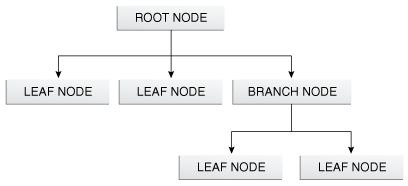
\includegraphics[width=0.45\textwidth]{grafiken/scenegraph2.png}
 \caption{Beispiel Szenegraph \cite{Hommel2013}}
 \label{fig:scenegraph2}
\end{figure} 
Jeder Standardknoten aus der JavaFX-Bibliothek implementiert ein Interface namens \textit{EventTarget}. Die Phasen, die ein Event durchläuft sind folgende:
\begin{enumerate}
	\item \textbf{Target selection:} Das Ziel des Events wird bestimmt (Bei Mausklick z.B. das Element, auf dem der Cursor ruht)
	\item \textbf{Route construction:} Die Route vom Wurzelknoten zum Ziel wird konstruiert
	\item \textbf{Event capturing:} Der Weg des Events vom Wurzelknoten zu dem Zielknoten
	\item \textbf{Event bubbling:} Der Weg des Events vom Zielknoten zurück zum Wurzelknoten
\end{enumerate}
Für das Eventhandling sind die Phasen \textit{Event Capturing} und \textit{Event Bubbling} die wichtigsten. Das Event \enquote{bewegt} sich auf der in Phase 2 konstruierten Route bis zum Zielknoten. Dabei passiert es zunächst den Wurzelknoten und weiterhin jeden Knoten, der im Baum des Szenegraphen zwischen diesem und dem Zielknoten liegt. Dies ist die \textit{Event Capturing} Phase. In der \textit{Event Bubbling} Phase nimmt das Event dann genau den umgekehrten Weg. Es bewegt sich vom Zielknoten zurück zum Wurzelknoten.\par
Das Event kann an jedem beliebigen Knoten bearbeitet werden, der auf dieser Route liegt. Soll ein Event in der \textit{Capturing}-Phase behandelt werden, muss ein Event-Filter an der entsprechenden Komponente registriert werden. Standardmäßig werden jedoch eher Event-Handler registriert, deren Code in der \textit{Bubbling}-Phase ausgeführt wird. Es ist durchaus möglich, einer Komponente mehrere Handler oder Filter hinzuzufügen, jedoch ist die Ausführungsreihenfolge innerhalb einer Phase nicht definiert. Zusätzlich gibt es \textit{Convenience}-Methoden, die das Hinzufügen eines \textit{Event-Handlers} vereinfachen, da der Typ des zu behandelnden Events nicht explizit angegeben werden muss. Zu beachten ist hierbei, dass die über die \textit{Convenience}-Methoden hinzugefügten Event-Handler pro Komponente erst nach den anderen Handlern ausgeführt werden und es nur genau einen pro Eventtyp gibt.\par
\begin{figure}[H]
 \centering
 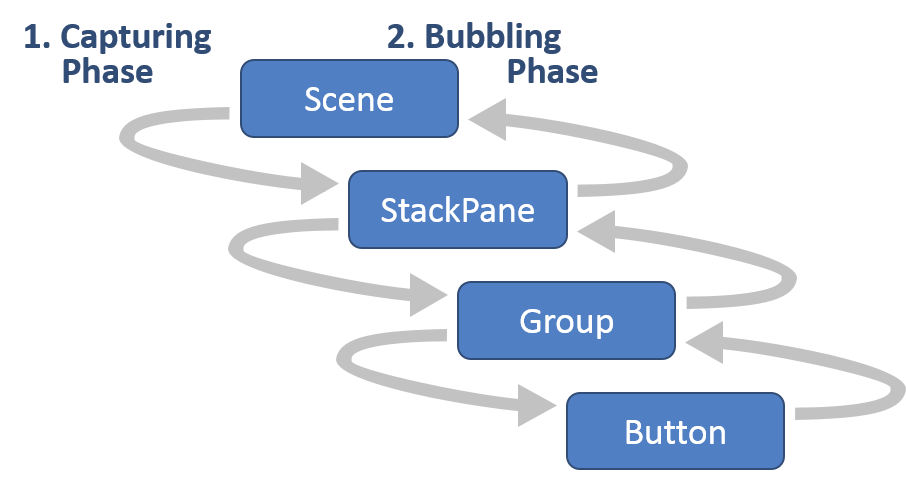
\includegraphics[width=0.75\textwidth]{grafiken/event_phase.png}
 \caption{Event Capturing und Bubbling}
 \label{fig:eventPhase}
\end{figure} 
Ist die Behandlung eines Events an einem bestimmten Knoten abgeschlossen, kann das Event entweder an den nächsten Knoten weitergereicht oder konsumiert werden. Wird das Event durch den Handler bzw. Filter konsumiert, wird es nicht weitergereicht und die Bearbeitung ist damit abgeschlossen.\par
\section{Die Anwendung \enquote{FalkoFX}} \label{sec:application}
Das Softwareprojekt \textit{Falko} beschäftigt sich mit der Visualisierung, Erstellung und Pflege länderspezifischer Fahrzeugdaten. Bei \textit{FalkoFX} handelt es sich um ein Unterprojekt für die Entwicklung eines weiteren Clients, der für einen Teil der Benutzer eine bessere Übersicht bietet und so eine höhere Produktivität ermöglicht. Das Projekt wird mit Java 8 und der JavaFX-Technologie umgesetzt.\par
Der FalkoFX-Client verfolgt, im Vergleich zu dem sehr umfangreichen Falko-Client, um einiges stärker den Ansatz der Usability. Neue Funktionalitäten werden zunächst fachlich durchgeplant und daraufhin mehrere Designkonzepte entworfen und vorgestellt. Moderne Bedienelemente, die von den Standardkomponenten zum Teil stark abweichen, wurden entworfen, um ein gutes, intuitives Nutzungsempfinden zu ermöglichen.\par
Das Software-System ist in verschiedene Anwendungsfälle untergliedert. Jeder Anwendungsfall hat ein eigenes zugrundeliegendes Datenmodell von Daten, die verglichen und aufbereitet angezeigt werden können. Wird über die Hauptnavigation in einen Anwendungsfall gewechselt, ist der erste Schritt das Auswählen der zu anzuzeigenden Daten. Dies geschieht über einen Filter, der anhand von Kriterien konfiguriert werden kann. Der nächste Schritt ist die Anzeige der Daten. In jedem Anwendungsfall stehen unterschiedliche Ergebnispräsentationen zur Verfügung, zwischen denen gewählt werden kann. Die verfügbaren Arten der Ergebnispräsentation begründen sich auf die Natur der unterliegenden Datenmodelle. Zu jedem in der Ergebnisansicht angezeigten Elemente können die Details aufgerufen werden.\par
\section{Responsive Design} %SubSection?
Das Responsive Design ist ein aus der Webentwicklung stammender Begriff. Es beschreibt die Fähigkeit einer Anwendung oder Webseite, auf verschiedenen Monitorgrößen darstellbar und benutzbar zu sein. So kann z.B. eine Webseite, die nach Richtlinien des Responsive Design erstellt wurde, sowohl auf einem Computermonitor (unabhängig von der Auflösung), als auch auf einem Tablet und einem Smartphone korrekt angezeigt werden.\par
\begin{figure}[H]
 \centering
 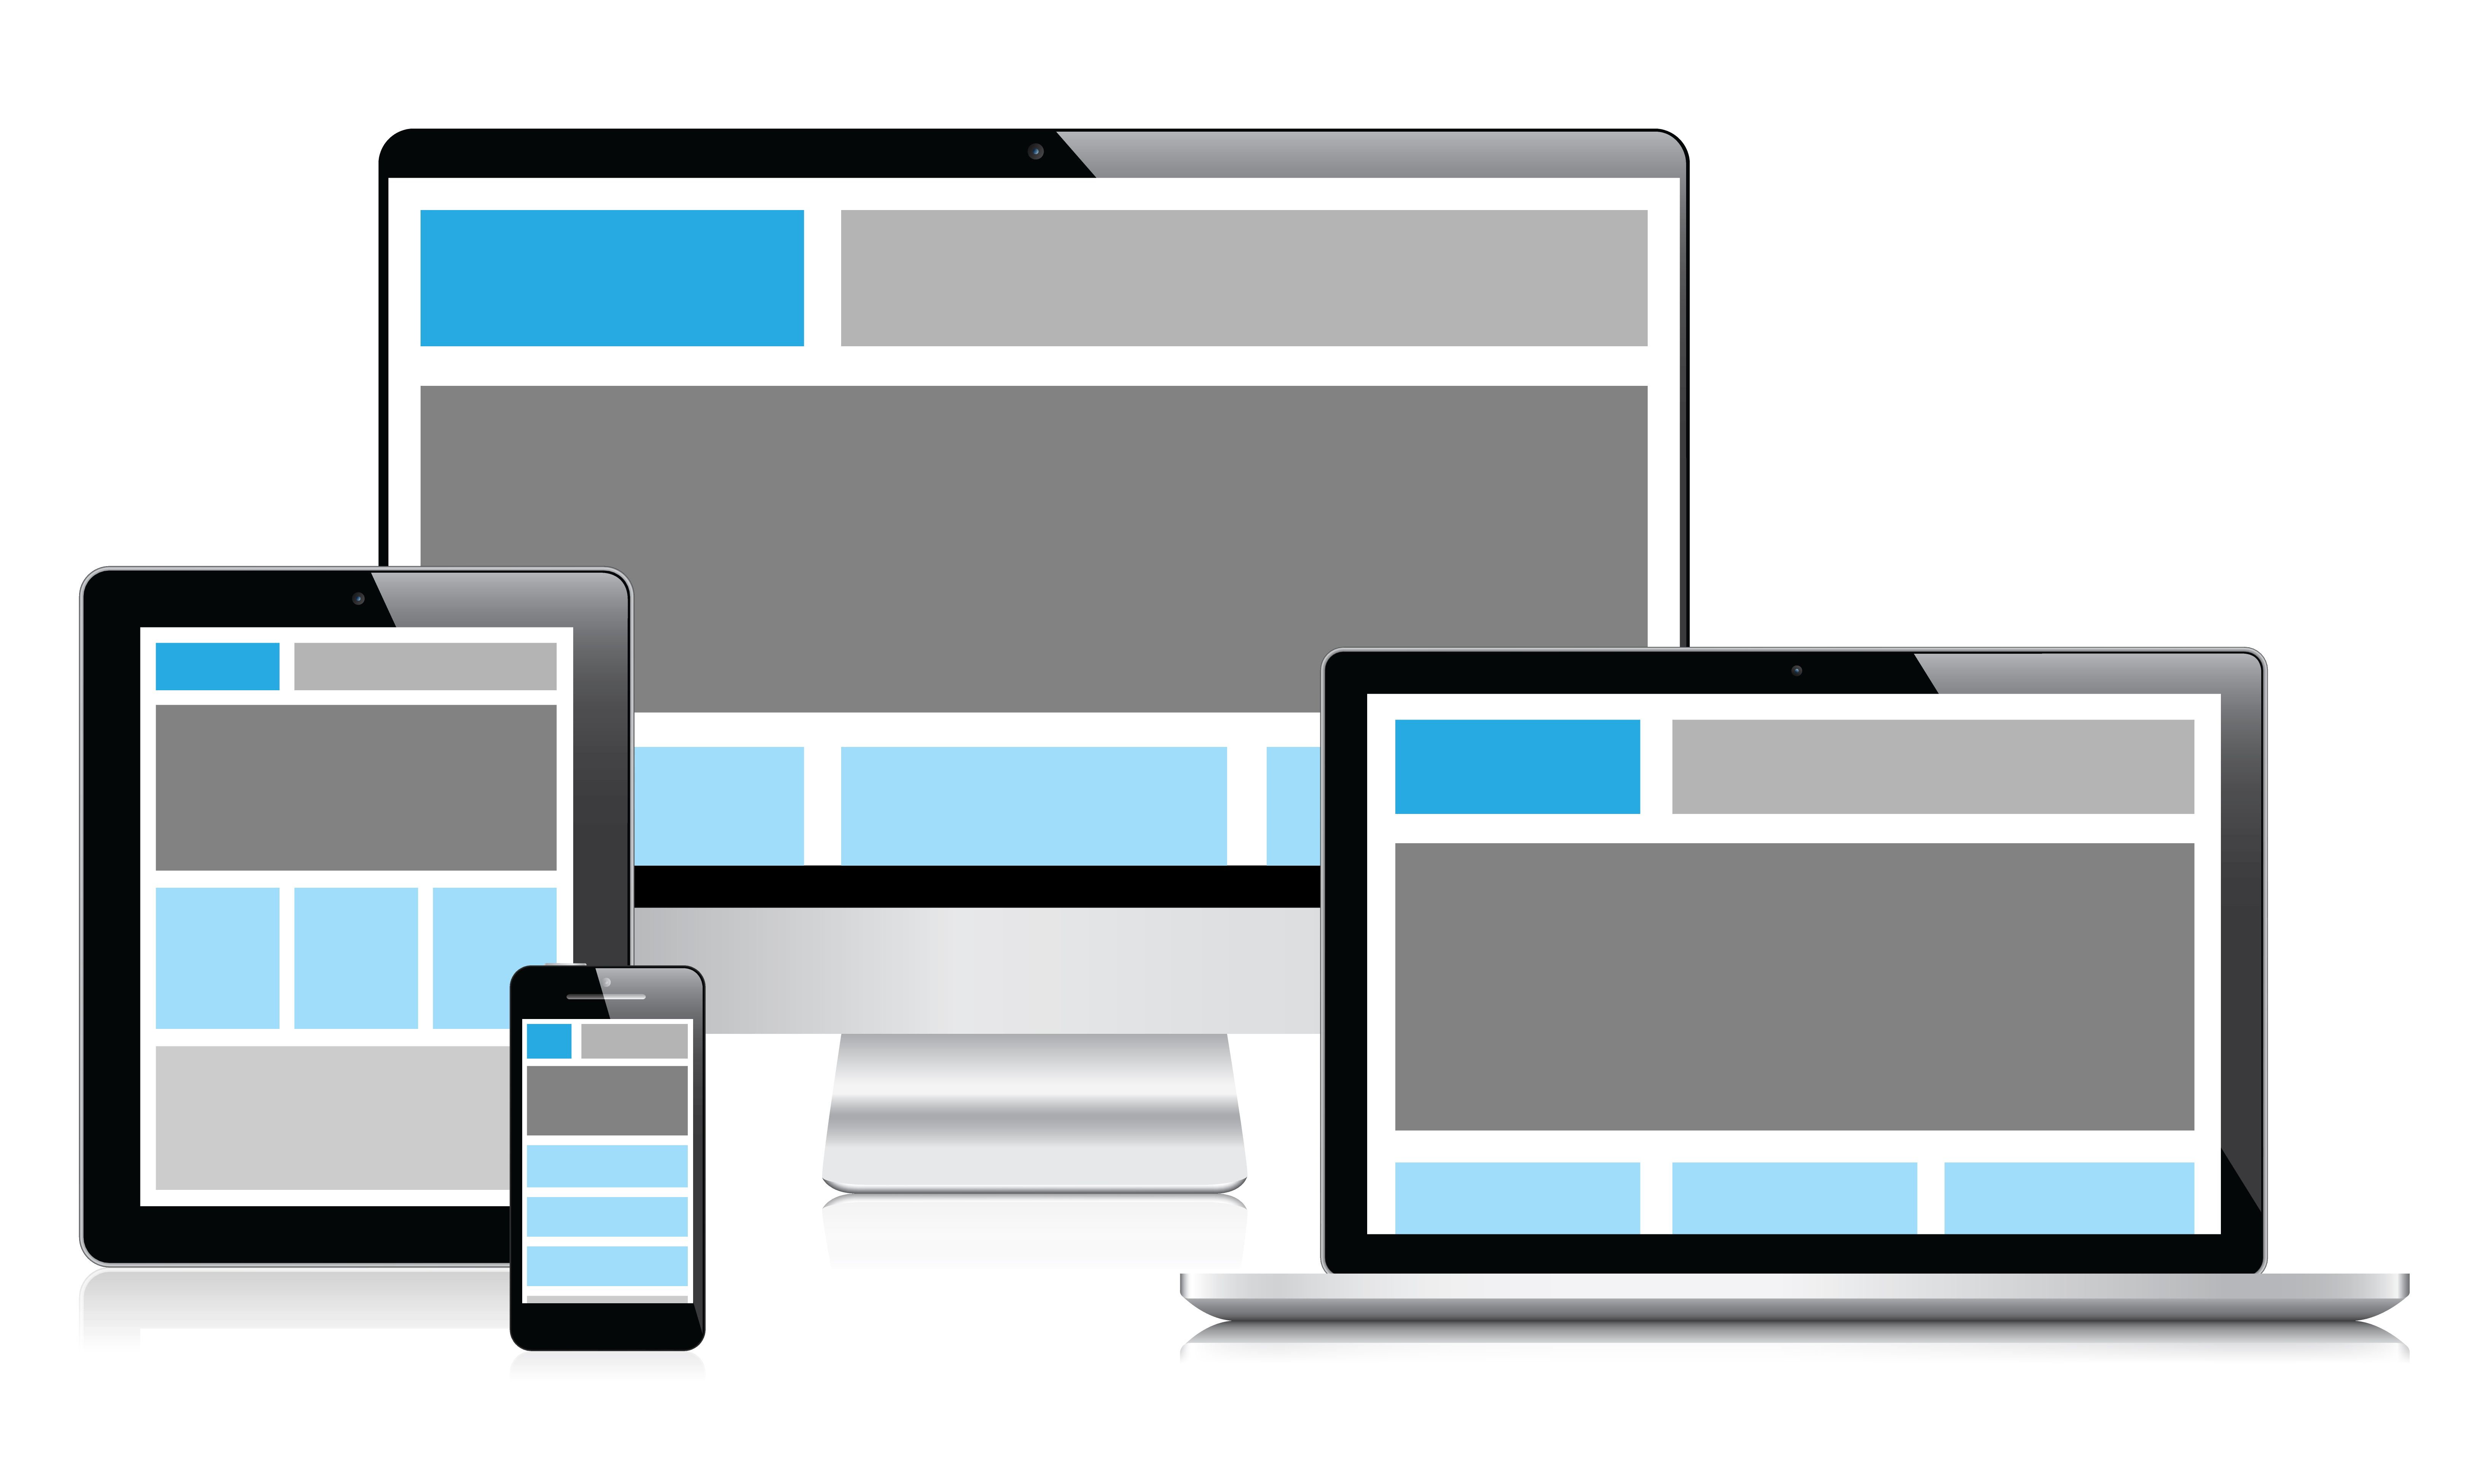
\includegraphics[width=0.5\textwidth]{grafiken/responsive_design.png}
 \caption{Beispiellayout Responsive Design \cite{Moon2013}}
 \label{fig:responsiveDesign}
\end{figure} 